% PRICAI 2026 compact submission version. Original full version is kept unchanged.
\documentclass[runningheads,orivec]{llncs}

\usepackage[T1]{fontenc}
\usepackage{amsmath,amssymb}
\usepackage{booktabs,multirow,array}
\usepackage{threeparttable}
\usepackage{graphicx}
\usepackage{hyperref}

\graphicspath{{../}}
\hypersetup{colorlinks=true,linkcolor=black,citecolor=black,urlcolor=blue,hypertexnames=false}
\emergencystretch=2em

\setlength{\textfloatsep}{6pt plus 1pt minus 2pt}
\setlength{\floatsep}{5pt plus 1pt minus 2pt}
\setlength{\intextsep}{5pt plus 1pt minus 2pt}
\setlength{\abovedisplayskip}{4pt plus 1pt minus 1pt}
\setlength{\belowdisplayskip}{4pt plus 1pt minus 1pt}
\setlength{\abovedisplayshortskip}{3pt plus 1pt minus 1pt}
\setlength{\belowdisplayshortskip}{3pt plus 1pt minus 1pt}
\renewcommand{\arraystretch}{1.04}

\newenvironment{tightitemize}{%
    \begin{itemize}\setlength{\itemsep}{1pt}\setlength{\parskip}{0pt}\setlength{\parsep}{0pt}}{\end{itemize}}
\newenvironment{tightenumerate}{%
    \begin{enumerate}\setlength{\itemsep}{1pt}\setlength{\parskip}{0pt}\setlength{\parsep}{0pt}}{\end{enumerate}}

\begin{document}

\title{Trust-Flow Trusted Federated Learning for Embodied AI Edge Collaboration}
\titlerunning{Trust-Flow-Driven Trusted Federated Learning}

\author{Anonymous Author(s)}
\authorrunning{Anonymous}
\institute{}

\maketitle

\begin{abstract}
    Federated learning (FL) supports collaborative embodied intelligence without moving raw sensory data, but open embodied devices expose aggregation to untrusted execution, model poisoning, stealthy backdoors, and severe Non-IID drift caused by physical-scene diversity. Existing robust aggregation often rejects attacks by also removing legitimate long-tail devices, while TEE-based admission alone cannot track runtime anomalies after admission. This paper proposes Trust Flow, a trusted FL framework for embodied AI edge collaboration. A trusted management and attestation agent (TMAA) turns TEE attestation, runtime monitoring, entropy features, and Kalman filtering into cross-round admission evidence. Trust Flow separates long-term utility from short-term attack risk, then applies layer-wise gating, dynamic clipping, and survivor weight re-normalization to suppress poisoned updates while preserving useful heterogeneous contributions. Flower/PyTorch experiments with CIFAR-10, 20 admitted embodied devices, six mixed attacks, and five repeated runs show 92.31\% accuracy and 10.21\% ASR under a 30\% malicious setting, with 0.00\% permanent-ban FPR in the tested configuration.
    \keywords{Federated Learning \and Embodied AI \and Edge Collaboration \and Trusted Execution Environment \and Risk Modeling \and Backdoor Defense}
\end{abstract}

\section{Introduction}

FL trains a global model through parameter exchange while keeping data on local devices \cite{kairouz2021flsurvey,mcmahan2017fedavg}. This design suits embodied AI edge collaboration, where devices collect privacy-sensitive sensory and interaction data. Open embodied networks require the server to judge update abnormality, device authenticity, execution integrity, runtime behavior, and semantic safety. They also exhibit sensor, task, mobility, and physical-scene heterogeneity, so robust aggregation must distinguish malicious deviations from legitimate long-tail updates. This distinction becomes harder under compound attacks, where adversaries may submit poisoned parameters, inject targeted backdoors, or exploit cross-round camouflage.

Prior work addresses different parts of this problem. Geometric and statistical defenses such as Krum and Trimmed Mean remove outlying updates \cite{blanchard2017krum,yin2018byzantine}. FLTrust and FoolsGold use clean references or temporal similarity \cite{cao2021fltrust,fung2020foolsgold}, while RaSA and FLDetector adapt aggregation or detection to edge-assisted and poisoning settings \cite{wang2025rasa,fldetector2022}. Backdoor-specific methods examine deep model behavior, clipping/noising, purification, or collusion patterns \cite{deepsight2022,flame2022,flpurifier}; related defenses further consider federated detection, targeted collusion, and privacy-preserving poisoning \cite{crowdguard2024,roseagg,shieldfl}. These mechanisms face two recurring tensions in embodied AI collaboration: software-side filtering cannot prove how local training was executed, and aggressive filtering often mistakes physical-scene Non-IID long-tail updates for attacks. TEE-based FL systems provide a hardware root of trust for integrity and SGX-based training \cite{r1_tee_integrity,xu2021distributed}; recent work further studies privacy-preserving FL, attack mitigation, and trustworthy training with malicious participants \cite{zhang2025rppfl,r5_tee_mitigating,lu2025tmt}. Yet TEE admission is usually a static gate and does not by itself solve semantic poisoning after admission.

This paper proposes \emph{Trust Flow}, a full-process trusted aggregation framework for embodied AI FL. Its key idea is to make trust evidence flow across admission, runtime monitoring, auditing, temporal state evolution, and aggregation. A device-side TMAA connects TEE attestation, runtime behavior, and dynamic trust evolution into a reusable admission signal. The contributions are:
\begin{tightenumerate}
    \item A TMAA-driven dynamic admission mechanism that combines TEE attestation, runtime behavioral entropy, and Kalman filtering into cross-round admission trust evidence.
    \item A dual-stream reputation model that decouples historical utility from short-term attack risk, reducing the tension between malicious recall and permanent false positives.
    \item A layer-wise risk-gated aggregation rule that applies differentiated admission thresholds, dynamic L2 clipping, and survivor weight re-normalization.
    \item An end-to-end embodied AI edge-collaboration evaluation under Non-IID CIFAR-10 and mixed attacks, with additional stress tests and ablations.
\end{tightenumerate}

\section{Background and Related Work}

\textbf{Federated learning for embodied AI edge collaboration.} In the standard FL workflow, devices complete local training and submit parameter updates to the server, which aggregates them and redistributes the global model. This workflow keeps data local but makes the server heavily dependent on the authenticity and quality of uploaded updates. Embodied AI further complicates this setting because devices differ in sensing modality, mobility pattern, compute capability, communication stability, task objective, and physical-scene distribution. A more open and layered system also increases the attack surface around device admission, local execution, and update aggregation.

\textbf{Poisoning and backdoor attacks.} Attacks in FL mainly include untargeted poisoning and targeted backdoors. Untargeted poisoning, such as sign flipping and gradient scaling, aims to disrupt convergence. Targeted attacks, including label flipping, trigger-based backdoors, clean-label poisoning, and semantic backdoors, try to preserve main-task behavior while implanting targeted misclassification. Backdoor attacks are especially challenging because a malicious update can remain close to normal directions while shifting hidden features \cite{bagdasaryan2020backdoor,wang2019neuralcleanse}. In a multi-round setting, attackers may also behave normally for several rounds to accumulate trust before injecting low-amplitude or intermittent malicious updates.

\textbf{Active defenses and their limits.} Robust aggregation methods typically rely on geometric distances, coordinate-wise statistics, clean anchors, temporal similarity, or adaptive aggregation. Krum and Trimmed Mean reject or suppress outlying updates \cite{blanchard2017krum,yin2018byzantine}; FLTrust uses a server-side clean reference direction \cite{cao2021fltrust}; FoolsGold and FLDetector exploit history or client behavior to identify malicious participation \cite{fung2020foolsgold,fldetector2022}; RaSA adapts secure aggregation under edge-assisted settings \cite{wang2025rasa}. Backdoor-oriented defenses inspect hidden behavior or update clusters \cite{deepsight2022,flame2022}, detect federated backdoors or collusion \cite{crowdguard2024,roseagg}, and mitigate poisoning through purification or privacy-preserving defense \cite{flpurifier,shieldfl}. These defenses remain sensitive to strong Non-IID distributions: a strict threshold raises benign false positives, whereas a loose threshold lets stealthy attacks pass.

\textbf{TEE-assisted trusted training.} Trusted execution environments (TEEs), including Intel SGX and ARM TrustZone, provide isolated execution and protected key material. Prior studies show their value in training integrity and SGX-based distributed learning \cite{r1_tee_integrity,xu2021distributed}, robust privacy-preserving FL and attack mitigation \cite{zhang2025rppfl,r5_tee_mitigating}, and trustworthy model training with malicious participants \cite{lu2025tmt}. Nevertheless, TEE admission alone cannot decide whether a genuine training process produced semantically safe model updates. Trust Flow therefore combines hardware-rooted admission with cross-round risk modeling and layer-aware robust aggregation.

\section{System Model and Threat Assumptions}

The system contains a central server $\mathcal{S}$ and $K$ embodied edge devices $\mathcal{C}=\{c_1,\ldots,c_K\}$. In round $t$, admitted devices receive $W^{(t-1)}$, train locally on sensory or interaction data, upload $\Delta W_k^{(t)}$, and the server updates $W^{(t)}=W^{(t-1)}+\mathrm{Agg}(\{\Delta W_k^{(t)}\})$. The global objective is
\begin{equation}
    \min_W \mathcal{L}(W)=\sum_{k=1}^{K}p_k\mathcal{L}_k(W),\quad
    p_k=|\mathcal{D}_k|/\sum_j|\mathcal{D}_j|.
\end{equation}
The embodied edge setting follows a device-edge-cloud workflow. The device side provides local training and trust evidence, while the server audits updates, evolves trust states, and performs secure aggregation.

\begin{figure}[t]
    \centering
    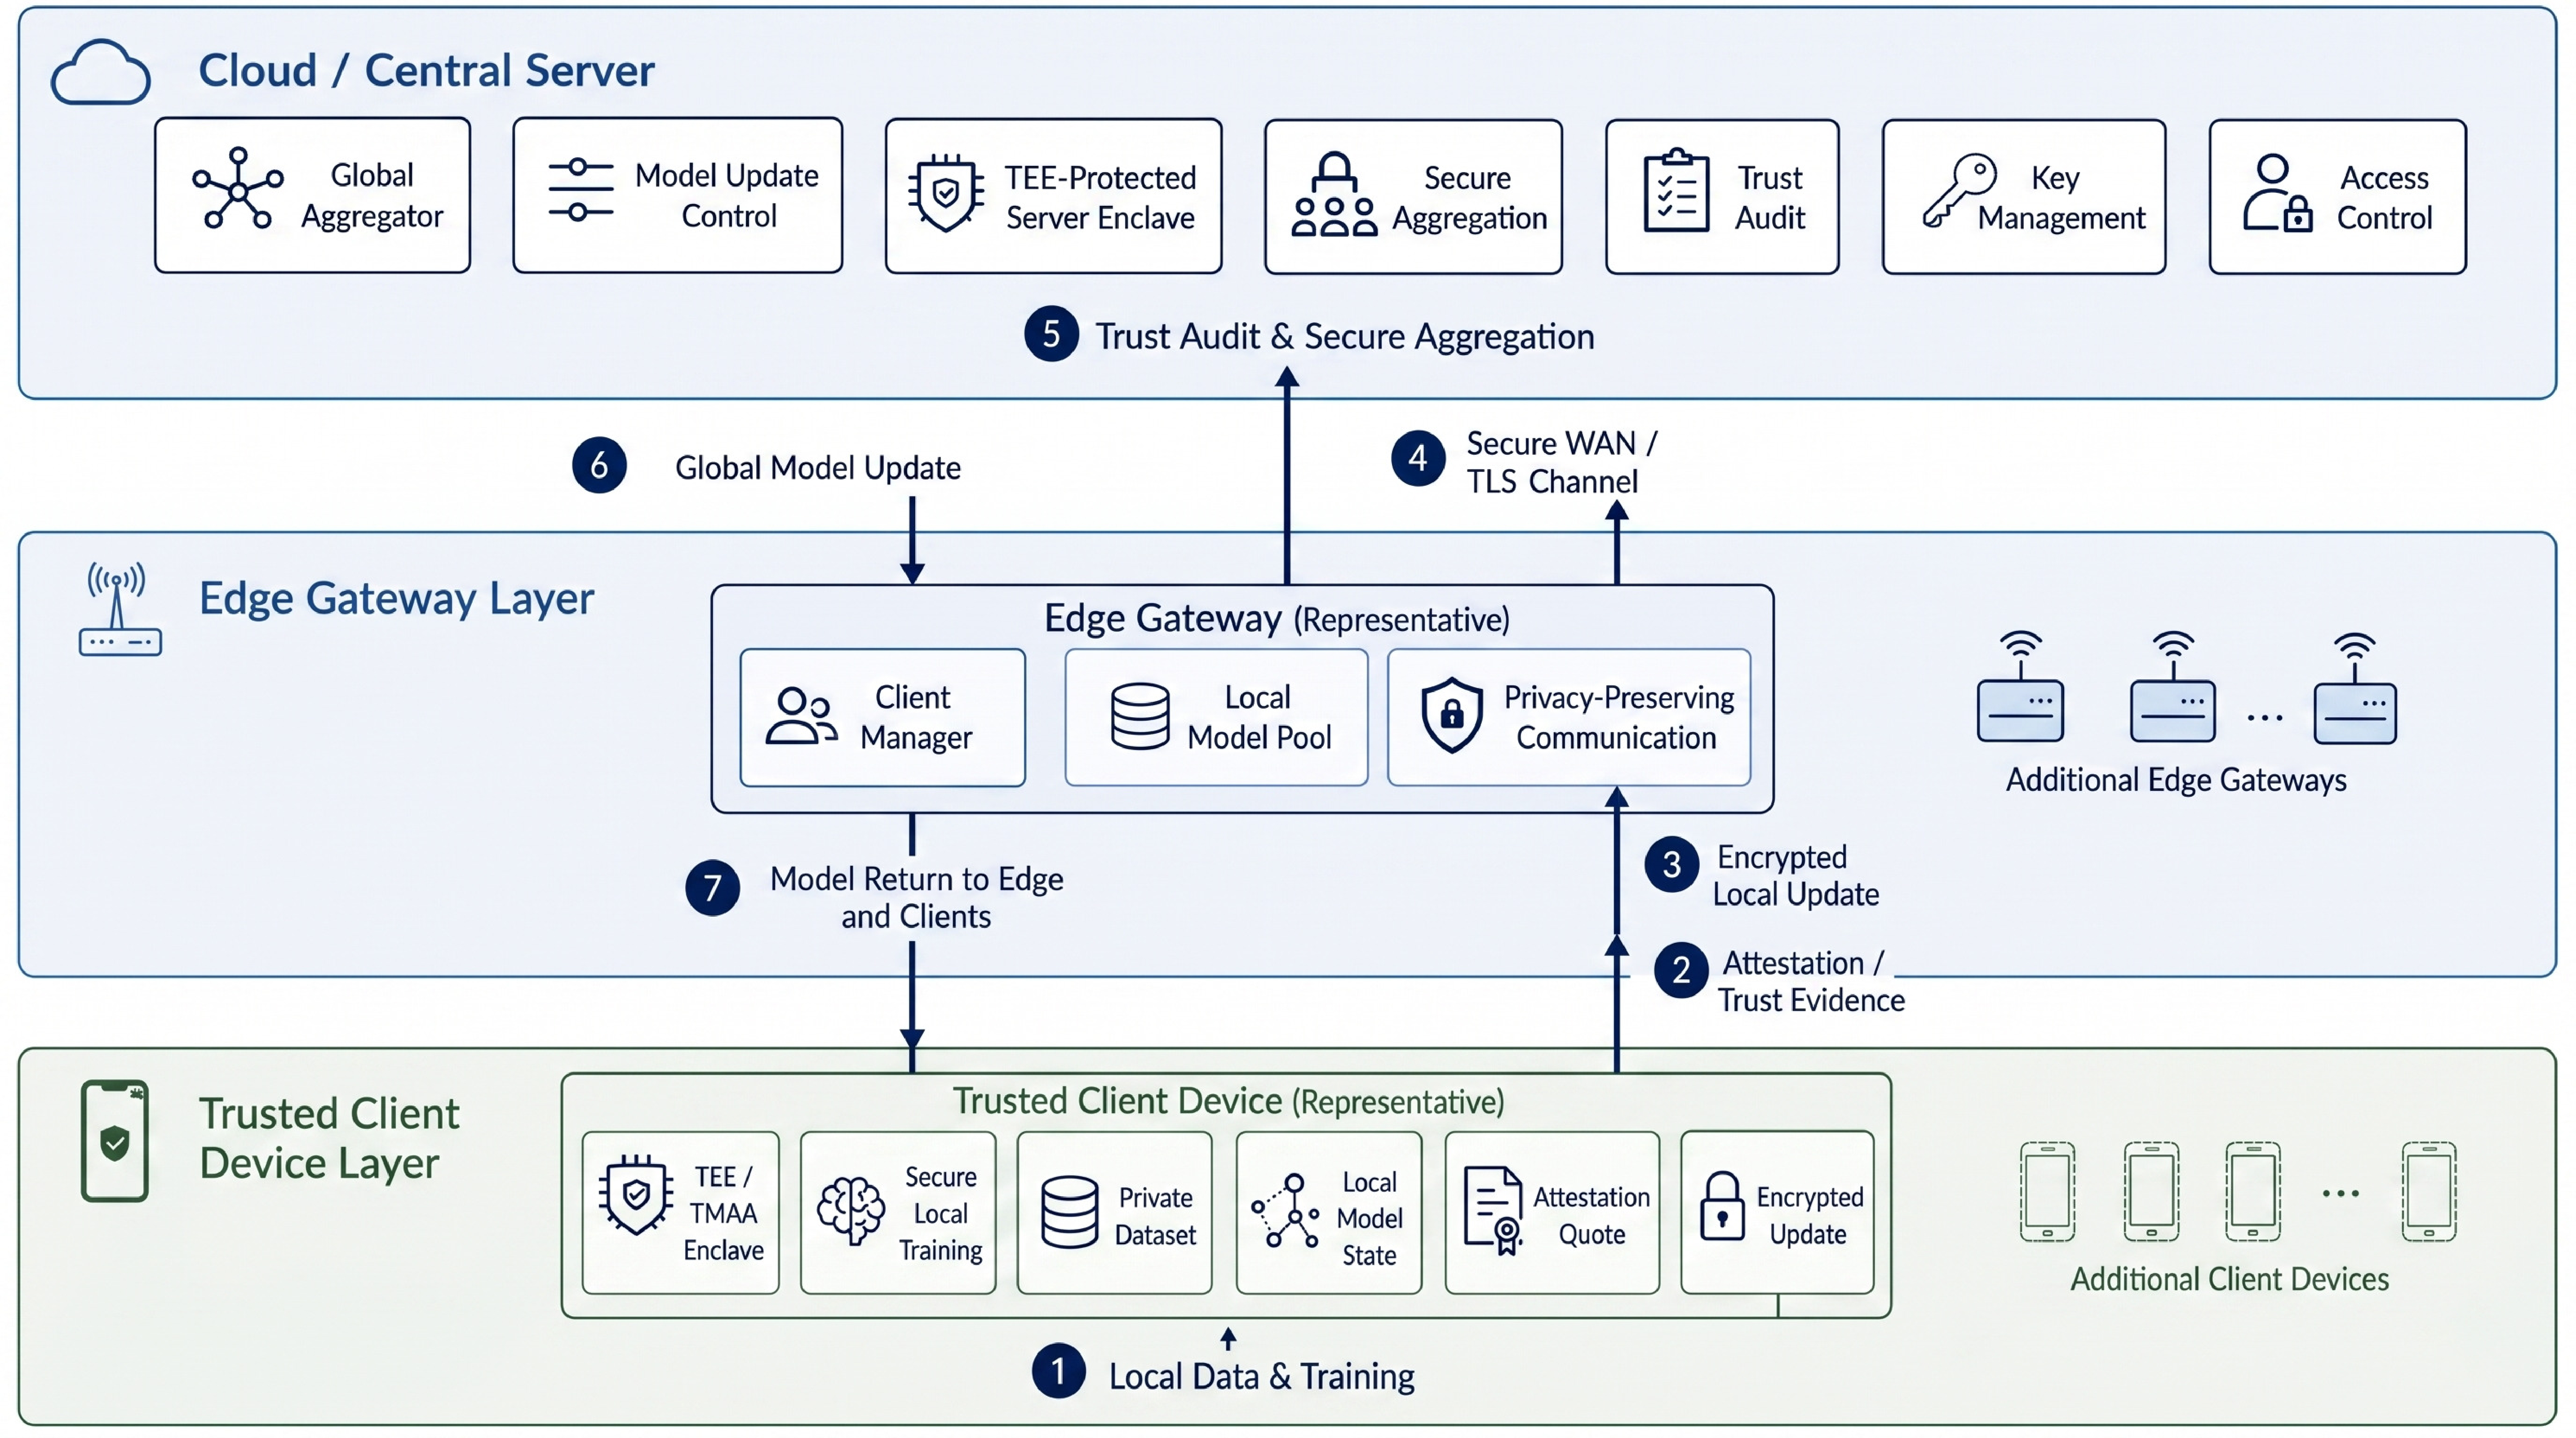
\includegraphics[width=0.84\textwidth]{fig1_system_arch.pdf}
    \caption{TEE-anchored embodied device-edge-cloud architecture.}
    \label{fig:system_arch}
\end{figure}

\begin{figure}[t]
    \centering
    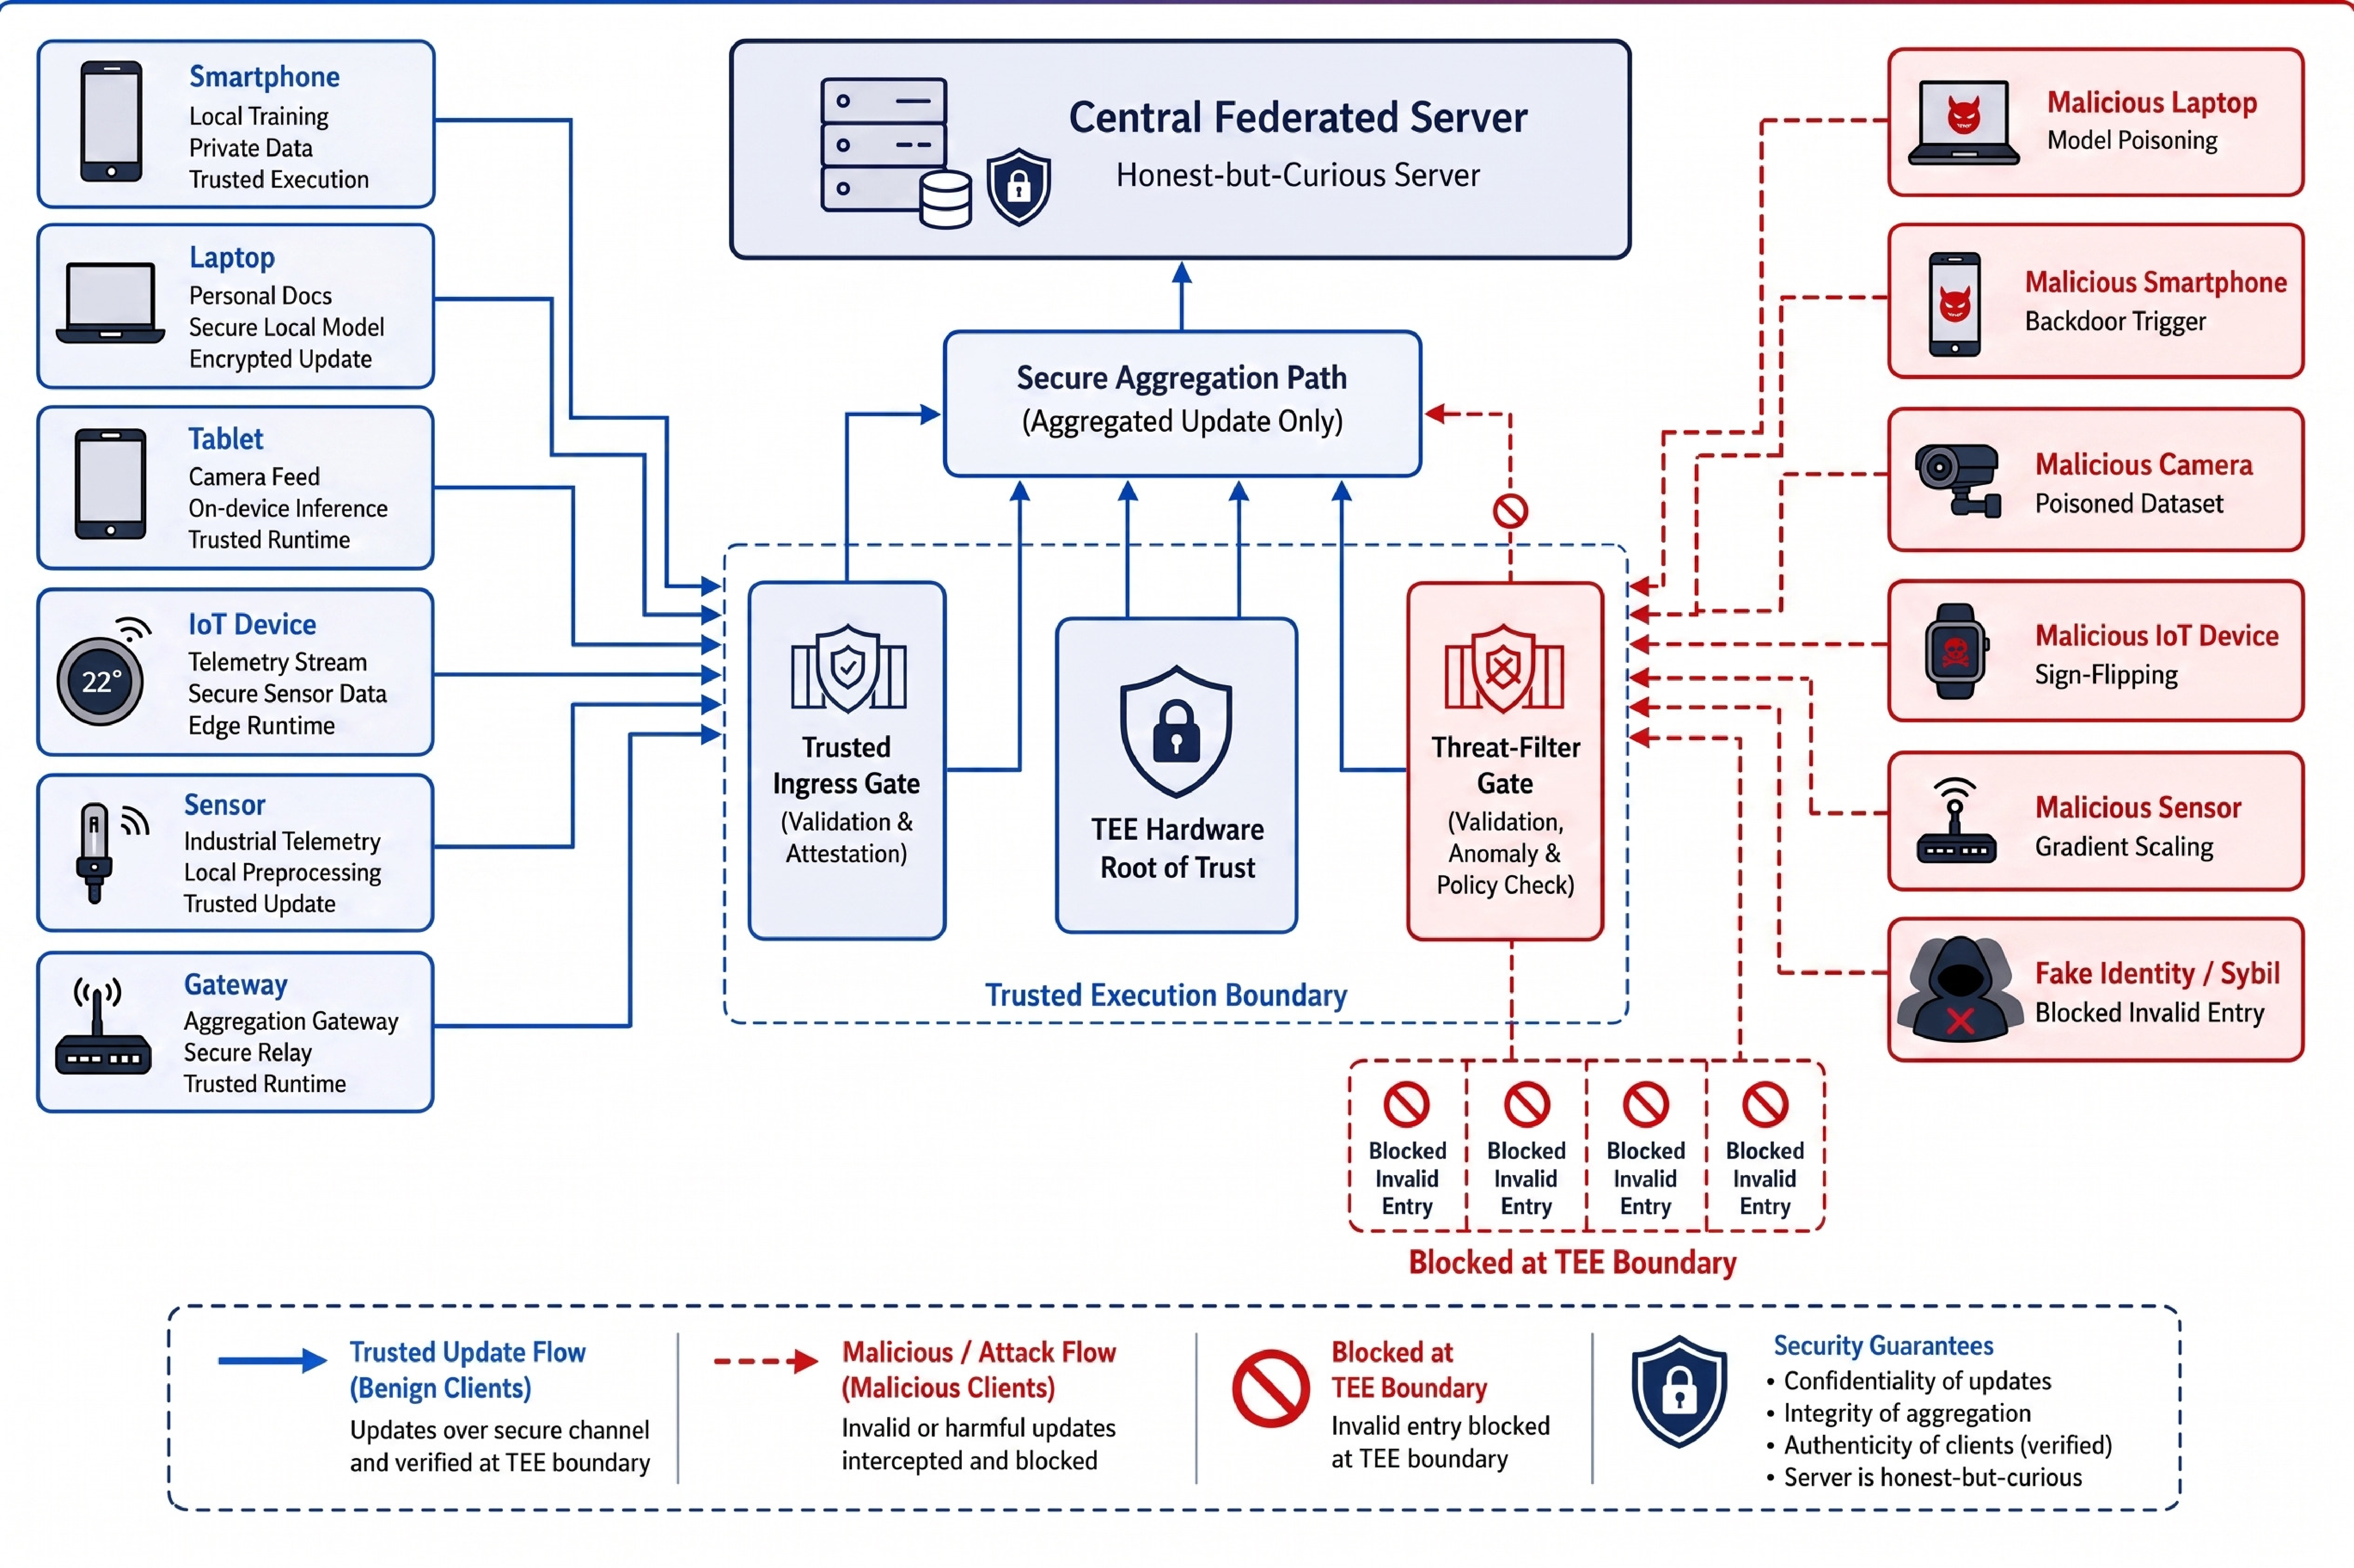
\includegraphics[width=0.80\textwidth]{fig2_threat_model.pdf}
    \caption{Composite poisoning and penetration threat model.}
    \label{fig:threat_model}
\end{figure}

\textbf{Threat model.} The server is honest-but-curious and follows the aggregation protocol. Attackers may control admitted embodied devices and perform label flipping, trigger backdoors, clean-label poisoning, semantic backdoors, sign flipping, and gradient scaling. This paper assumes an upper bound of $<50\%$ malicious devices. The main experiments use 30\% as a typical high-risk setting and additionally report a 50\% boundary stress test. TEEs are assumed to protect attestation-critical code and keys against a compromised host OS, excluding physical probing and advanced microarchitectural side-channel attacks.

\textbf{Design goals.} Trust Flow is designed to: (i) maintain convergence under mixed poisoning and backdoors; (ii) keep the FPR for permanent bans low for legitimate long-tail embodied devices; and (iii) avoid heavyweight cryptographic overhead while preserving edge deployability. Figures~\ref{fig:system_arch} and \ref{fig:threat_model} summarize the physical workflow and the threat surface.

The central difficulty is that these goals are coupled. In a pure filtering strategy, strengthening the rejection rule improves malicious recall but also removes benign devices whose local distributions deviate from the majority. Conversely, relaxing the rule protects long-tail devices but allows low-amplitude poisoning to persist. Trust Flow treats this as a state-separation problem rather than a threshold-tuning problem: admission evidence, content quality, historical contribution, and short-term risk remain visible as different signals until the final layer-wise aggregation decision.

\section{Trust-Flow Framework}

Trust Flow divides each FL round into four linked stages: admission and runtime trust assessment, reference-based content auditing, dual-stream state evolution, and risk-gated layered aggregation. Figure~\ref{fig:framework} shows the full defense loop.

\begin{figure}[t]
    \centering
    
\includegraphics[width=0.86\textwidth]{fig3_arch.pdf}
    \caption{Overview of the trust-flow defense loop for embodied AI collaboration.}
    \label{fig:framework}
\end{figure}

At a higher level, the framework is a trust-state transfer pipeline. Phase one outputs $TrustScore$, which captures whether the device has a trustworthy basis for participation. Phase two outputs $ContentScore$, which measures whether the current update agrees with the clean reference and the peer group. Phase three deposits these signals into $HistPerf$ and $RiskEMA$, separating long-term contribution from short-term abnormality. Phase four fuses the states into $RawScore$ and performs differentiated layer-wise aggregation. This design avoids treating a low single-round score as immediate evidence of maliciousness, which is important for long-tail devices under strong Non-IID data.

Operationally, each round follows the same decision path. The server first removes devices that fail the admission proof, since their updates cannot be tied to a protected execution path. It then scores the remaining updates against the clean reference and the trusted peer group, but still treats this score as provisional. The provisional evidence is accumulated into slow utility and fast risk states, and only then translated into layer-level aggregation privileges. This ordering is deliberate: early stages ask whether the evidence is credible, middle stages ask whether the current update is useful or risky, and the final stage asks where in the network the update should be allowed to contribute. The framework therefore avoids a single hard gate at the beginning of the round, which would be brittle under Non-IID data, while still enforcing hard isolation when risk evidence persists.

\subsection{Admission and Content Auditing}

Each admitted embodied device must pass a TEE-style admission check. Let $M_{\text{attest},k}\in\{0,1\}$ denote whether the attestation report is valid. During initialization, the device invokes a device-unique key and generates a remote attestation quote that includes integrity measurements such as PCR chains, code segment signatures, and runtime configuration. Only devices passing this check receive communication privileges. During local training, the trusted management agent monitors behavioral sequences
$\mathcal{X}_k=\{\Delta\text{grad},\Delta\text{loss},\text{instr\_dist}\}$. Their entropy, $H(\mathcal{X}_k)=-\sum_i p(x_i)\log p(x_i)$, is mapped to a measurement uncertainty $R_k^{(t)}=\exp(\lambda H(\mathcal{X}_k^{(t)}))$. Intuitively, a device whose local training suddenly becomes high-entropy is not necessarily malicious, but its current evidence should be trusted less than evidence produced under stable execution.

Following a robust filtering view, the trust estimate is updated as
\begin{equation}
    \hat{T}_{k}^{(t)}=\hat{T}_{k}^{(t-1)}+K_k^{(t)}(Z_k^{(t)}-\hat{T}_{k}^{(t-1)}),\quad
    TrustScore_k=\hat{T}_{k}^{(t)}(1+P_k^{(t)})^{-1}.
\end{equation}
High-entropy runtime behavior therefore reduces the Kalman gain and prevents abrupt anomalous observations from being absorbed into the long-term trust estimate. The covariance $P_k^{(t)}$ serves as a confidence boundary: smaller covariance indicates more reliable trust estimation. Thus admission is not a one-time binary decision, but a continuously updated privilege factor that can be carried into later auditing and aggregation.

The server then constructs a clean guiding direction. If a small clean validation gradient is available, $g_{root}=g_{root\_clean}$; otherwise, it uses admitted devices with high trust and low previous risk, with reference weights $\omega_k^{ref}=TrustScore_k(1-RiskEMA_k^{prev})^2$. This fallback matters in embodied deployments where a server-side clean set may be small or absent: the reference should be conservative, but it should not be dominated by devices that were recently suspicious. For each update, content quality combines reference consistency and peer consistency:
\begin{align}
    S_{contrib,k}  & =\max(0,\alpha_1+\alpha_2\cos(\Delta W_k,g_{root})),                                  \\
    S_{consist,k}  & =\frac{\sum_{j\ne k}TrustScore_j\max(0,\alpha_1+\alpha_2\cos(\Delta W_k,\Delta W_j))}
    {\sum_{j\ne k}TrustScore_j+\varepsilon},                                                               \\
    ContentScore_k & =\frac{(1+\beta_{fusion}^2)S_{consist,k}S_{contrib,k}}
    {\beta_{fusion}^2S_{consist,k}+S_{contrib,k}+\varepsilon}.
\end{align}
Here $\beta_{fusion}>1$ increases the influence of the clean direction and helps resist collusive drift. The harmonic form is used deliberately: a device must be plausible both relative to the clean reference and relative to the trusted peer group. A high peer score alone is insufficient under collusion, while a high reference score alone may over-penalize legitimate Non-IID updates.

\subsection{Dual-Stream State Evolution}

Single reputation scores confuse low utility caused by data skew with high risk caused by attacks. Trust Flow therefore separates device state into a historical utility stream and a short-term risk stream. The historical stream treats normalized content quality as soft evidence in a Beta reputation model. Good evidence increases $\alpha_k$, weak evidence increases $\beta_k$, both with decay $\lambda_h$, and the expected historical utility is $HistPerf_k^{(t)}=\alpha_k^{(t)}/(\alpha_k^{(t)}+\beta_k^{(t)}+\varepsilon)$.

This channel is intentionally slow. A legitimate long-tail embodied device may receive a low content score in a few rounds because its scene distribution differs from the majority, not because it is attacking the model. A low $HistPerf$ therefore leads to reduced aggregation privilege or temporary soft isolation, rather than immediate permanent removal. The risk stream plays the opposite role. It takes the maximum over several probes, including report anomalies, gradient direction/amplitude, clean-set loss increase, trigger activation drift, sign inconsistency, and peer disagreement, and then updates $RiskEMA_k^{(t)}=\beta_rRiskEMA_k^{(t-1)}+(1-\beta_r)Risk_k^{inst}$. A single strong attack signal is therefore not averaged away by benign historical behavior.

The separation also changes how borderline devices are treated. A device with weak content quality but no rising risk is kept in the system with reduced influence, giving later rounds a chance to confirm whether the low score was caused by Non-IID drift. A device with moderate historical utility but a sudden risk spike is handled in the opposite way: its current update is down-weighted or blocked before it can enter sensitive layers. This asymmetric response explains the low permanent-ban FPR observed in the tested configuration, because the framework does not require the same threshold to serve as both a quality filter and an attack detector.

The two streams meet only when computing aggregation privilege:
\begin{align}
    RawScore_k & = (TrustScore_k)^\alpha(ContentScore_k)^\beta
    (HistPerf_k^{(t-1)})^\gamma \nonumber                      \\
               & \quad \times (1-RiskEMA_k^{(t-1)})^p .
\end{align}
The multiplicative form makes the final privilege conservative: a device needs sufficient execution trust, current content quality, historical utility, and low recent risk. The resulting state machine distinguishes NORMAL, SUSPECT, QUARANTINE, and BLACKLIST states, as shown in Fig.~\ref{fig:state_machine}. A sleeper-burst attacker may accumulate high $HistPerf$ during early benign rounds, but a later trigger injection activates the trigger or clean-probe channels and increases $RiskEMA$, blocking the attack even when historical utility is high. Conversely, a long-tail benign device with low current similarity is mainly handled through the slow utility stream and can recover after later positive contributions.

\begin{figure}[t]
    \centering
    
\includegraphics[width=0.76\textwidth]{fig4_state.pdf}
    \caption{Client state-transition automaton driven by historical utility and short-term risk.}
    \label{fig:state_machine}
\end{figure}

\subsection{Risk-Gated Layered Aggregation}

Backdoors often concentrate in deeper layers, whereas shallow feature layers may carry useful heterogeneous information. Trust Flow therefore assigns each layer $l$ a sensitivity score:
\begin{figure}[t]
    \centering
    
\includegraphics[width=0.78\textwidth]{fig5_layer.pdf}
    \caption{Risk-gated layer-wise clipping and differentiated aggregation.}
    \label{fig:layer_gating}
\end{figure}
The score combines three signals: privacy exposure, reference-gradient utility, and security deviation. The privacy term decays with depth, the utility term measures the relative reference-gradient norm of the layer, and the security term measures how far trusted device updates drift from the reference direction. Their weighted sum $S_{total}^{(l)}$ controls both the admission threshold $\theta^{(l)}=\mu_{base}+\lambda_sS_{total}^{(l)}$ and the clipping radius $C^{(l)}=C_{base}/(S_{total}^{(l)}+\varepsilon_c)$. Thus a layer with stronger suspicious drift becomes harder to enter and more tightly clipped; a layer that remains close to the reference keeps more capacity for benign heterogeneity.

Survivors are $\Phi^{(l)}=\{k\in\mathcal{A}\mid RawScore_k\ge\theta^{(l)}\}$, and their weights are re-normalized:
\begin{equation}
    \tilde{w}_{k}^{(l)}=\frac{RawScore_k}{\sum_{j\in\Phi^{(l)}}RawScore_j+\varepsilon},\quad
    \widehat{\Delta W}_k^{(l)}=\frac{\Delta W_k^{(l)}}{\max(1,\|\Delta W_k^{(l)}\|_2/C^{(l)})}.
\end{equation}
The final update is $\Delta W_{global}^{(l)}=\sum_{k\in\Phi^{(l)}}\tilde{w}_{k}^{(l)}\widehat{\Delta W}_k^{(l)}$. Weight re-normalization prevents the removal of risky devices from shrinking the effective learning rate.

This layer-wise control is intended to preserve useful shallow representations while hardening layers that show stronger attack sensitivity. Consider a semantic backdoor that mainly shifts the final classifier or deep feature layers: a uniform global clipping rule must either be loose enough to preserve shallow features or tight enough to suppress the deep-layer attack, but it cannot do both well. Trust Flow allows those layers to follow different policies in the same round. The deep layer can reject low-privilege devices and reduce the update radius, while shallow layers still use permissive thresholds when their reference consistency remains stable. This differentiated treatment is important because a uniform clipping radius can over-suppress benign feature extraction layers and slow convergence, especially after malicious devices have already been removed from the survivor set.

The re-normalization step is equally important for convergence. Without it, removing suspicious devices would reduce the sum of effective aggregation weights and create an implicit learning-rate decay. That decay is easy to overlook because it appears as a robustness decision, but it directly slows optimization under a fixed 30-round budget. Trust Flow therefore treats filtering and optimization as coupled operations: once the unsafe mass is removed, the remaining trustworthy mass is projected back to a valid aggregation simplex before clipping and layer assembly.

\subsection{Analytical View}

The dual-stream structure gives a simple way to interpret the FPR/ASR tradeoff. Suppose the single-round content score of a legitimate long-tail device follows a perturbed distribution with expectation $\mu_{clean}$ and variance $\sigma_{clean}^2$. A rigid threshold can eliminate this device whenever its current score is below the threshold, even if the deviation comes from Non-IID data. After exponential smoothing, the steady-state variance of the historical utility estimate follows the standard low-pass form:
\begin{equation}
    \operatorname{Var}(HistPerf_k^{(\infty)})=\frac{1-\beta_h}{1+\beta_h}\sigma_{clean}^2 .
\end{equation}
As $\beta_h$ approaches 1, short-term benign fluctuations are suppressed and the device is less likely to face sustained removal. In contrast, the short-term risk stream responds to attack impulses. If a backdoor round produces an abnormal probe value, the max operator prevents that event from being averaged away before entering the EMA. Processing long-term contribution and short-term risk in separate spaces therefore reduces the single-score conflict: long-tail updates are smoothed rather than banned immediately, while abrupt malicious signals retain enough strength to trigger isolation.

\subsection{Risk Probe Computation}

The short-term risk stream uses probes that are intentionally redundant rather than individually decisive. The gradient probe measures both direction deviation from $g_{root}$ and abnormal update magnitude relative to the round statistics. This catches sign flipping and gradient scaling, but it is not sufficient for clean-label attacks whose directions may remain close to benign updates. The clean probe therefore applies a candidate update to a small server-side probe set and records the increase in cross-entropy loss. The trigger probe compares high-level activation histograms using KL divergence, $r_{trigger,k}^{(t)}=\mathrm{KL}(\mathcal{H}(A_{base})\|\mathcal{H}(A_k))$, which is more sensitive to semantic or clean-label backdoors that leave low-level gradients nearly unchanged.

These probes are fused through a maximum rule because their failure modes differ. A high-amplitude attacker is usually exposed by the gradient channel before it affects validation loss. A stealthy backdoor may instead appear as a modest clean-loss change but a clear activation shift. By preserving the strongest current warning, the risk stream makes each attack family visible to the state machine without requiring a single universal anomaly score.

The probes also provide useful diagnostic roles during auditing. When the gradient channel dominates, the server treats the device as an optimization-level threat and mainly suppresses its influence through clipping and layer thresholds. When the clean or trigger channel dominates, the update may look numerically ordinary but semantically unsafe, so the state machine pushes the device toward quarantine even if its historical utility is high. Peer disagreement is used as supporting evidence rather than a standalone reason for removal, because legitimate long-tail devices can disagree with the majority. This diagnostic separation makes the defense less dependent on a single score calibration and helps explain why the same mechanism can handle explicit parameter attacks, clean-label drift, and semantic backdoors in one pipeline.

\section{Experiments}

\subsection{Setup}

Experiments use Flower 1.5.0 and PyTorch on CIFAR-10 with a lightweight CNN to emulate distributed visual perception across embodied edge devices. Simulations are deployed on an Inspur server with dual CPUs and five NVIDIA A10 GPUs. The software stack is Ubuntu 20.04.6 LTS and CUDA 12.8. To support reproducibility, complete logs, source code, and startup scripts are preserved. The 50,000 training images are split among 20 admitted devices. A shared 5,000-sample balanced pool supplies a common alignment basis; devices 6--11 follow Dirichlet $\alpha=1.0$, and devices 12--19 use strong long-tail partitions with $\alpha=0.1$.

The formal 30\% attack setting uses six malicious devices: Client 0 performs label flipping with $\gamma=0.5$; Client 1 injects a trigger backdoor into 20\% of samples and targets class 0; Client 2 uses clean-label backdoor perturbations; Client 3 uses semantic backdoor bias; Client 4 applies sign flipping; and Client 5 amplifies updates by a factor of 100. Five Sybil devices without valid certificates and three free-rider devices with forged low workload are used to validate Phase-One gating. These eight devices are intercepted before the statistical analysis, so the later metrics are computed over the 20 admitted devices. Each run uses 30 rounds and three local epochs. Aggregate Acc/ASR values are averaged over five seeds; state trajectories are shown from one representative seed.

Accuracy and ASR are reported as mean and standard deviation over five independent runs. Permanent-ban FPR is computed over benign devices that are irreversibly blacklisted, while temporary SUSPECT or QUARANTINE states are treated as recoverable control actions. The single-run trajectory figures are taken from a fixed seed to make device-level transitions readable; aggregate tables use the repeated runs. All baselines are executed under the same device partitioning, attack proportion, optimizer configuration, communication rounds, and Non-IID split.

\begin{table}[t]
    \centering
    \caption{Compact experimental configuration and main hyperparameters.}
    \label{tab:setup}
    \small
    \begin{tabular*}{\textwidth}{@{\extracolsep{\fill}} p{2.45cm} p{5.2cm} p{4.25cm}}
        \toprule
        Category & Setting & Value \\
        \midrule
        FL task & Dataset/model/admitted devices & CIFAR-10/light CNN/$K=20$ \\
        Optimization & Local epochs, lr, momentum, rounds & $3$, $0.001$, $0.9$, $30$ \\
        Data heterogeneity & Shared pool, Group A, Group B/C & $5000$, $\alpha=1.0$, $\alpha=0.1$ \\
        Trust streams & $\alpha_1,\alpha_2,\beta_{fusion}$; $\beta_h,\beta_r$ & $0.6,0.4,2.0$; $0.9,0.85$ \\
        Layer gating & fusion exponents; $\mu_{base},\lambda_s$ & $3.0,1.0,0.5,1.0$; $0.4,1.2$ \\
        \bottomrule
    \end{tabular*}
\end{table}

\subsection{Overall Defense Performance}

Figure~\ref{fig:main_results} summarizes convergence, ASR, trust-state trajectories, and feature separation. Under 30\% mixed attacks, Trust Flow converges to 92.31\% accuracy and reduces ASR to 10.21\%, close to the random-guess baseline for CIFAR-10. Device-state tracing shows that explicit poisoning and parameter attacks are blocked early, while stealthier clean-label drift is captured after persistent probe evidence. Legitimate long-tail devices may enter SUSPECT or QUARANTINE temporarily, but their risk stream does not accumulate enough evidence for permanent banning.

The device trajectories expose different decision paths. Label flipping and trigger backdoor devices show sustained high $r_{grad}$ and $r_{probe}$ values and enter the blacklist by round 8. Semantic backdoor behavior first causes soft isolation and then removal after persistent risk accumulation. The clean-label attacker is harder to detect because its local loss appears normal; it is identified after the drift-combination rule remains active for several rounds. Sign flipping sharply reduces the directional contribution score, whereas gradient scaling is caught by amplitude and layer-wise clipping. In contrast, the long-tail legitimate device may show low content quality early, but its risk stream does not keep rising, allowing it to recover through later $HistPerf$ updates.

The t-SNE visualization provides a complementary view. Before trust-flow intervention, malicious and legitimate long-tail devices can occupy overlapping regions because both may deviate from the majority direction. After dual-stream supervision, malicious devices form separable clusters associated with high-risk probes, whereas legitimate long-tail devices remain connected to the main aggregation region. This supports the design claim that historical utility and short-term risk should not be collapsed into one score too early.

\begin{figure}[t]
    \centering
    \begin{minipage}{0.49\textwidth}
        \centering
        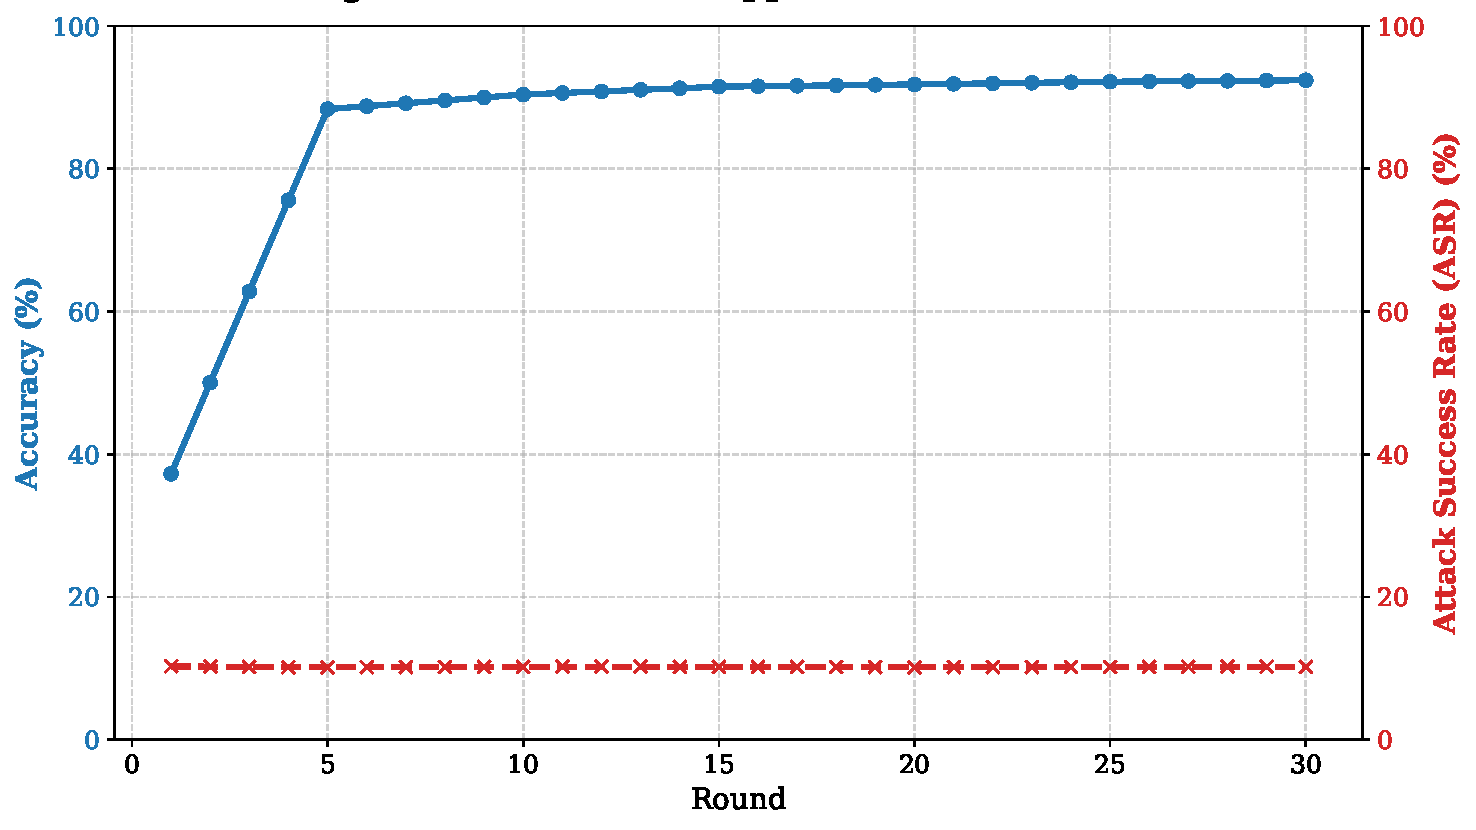
\includegraphics[width=\linewidth]{fig6_convergence_asr.pdf}
        \vspace{-3pt}
        {\scriptsize (a) Accuracy and ASR convergence.}
    \end{minipage}\hfill
    \begin{minipage}{0.49\textwidth}
        \centering
        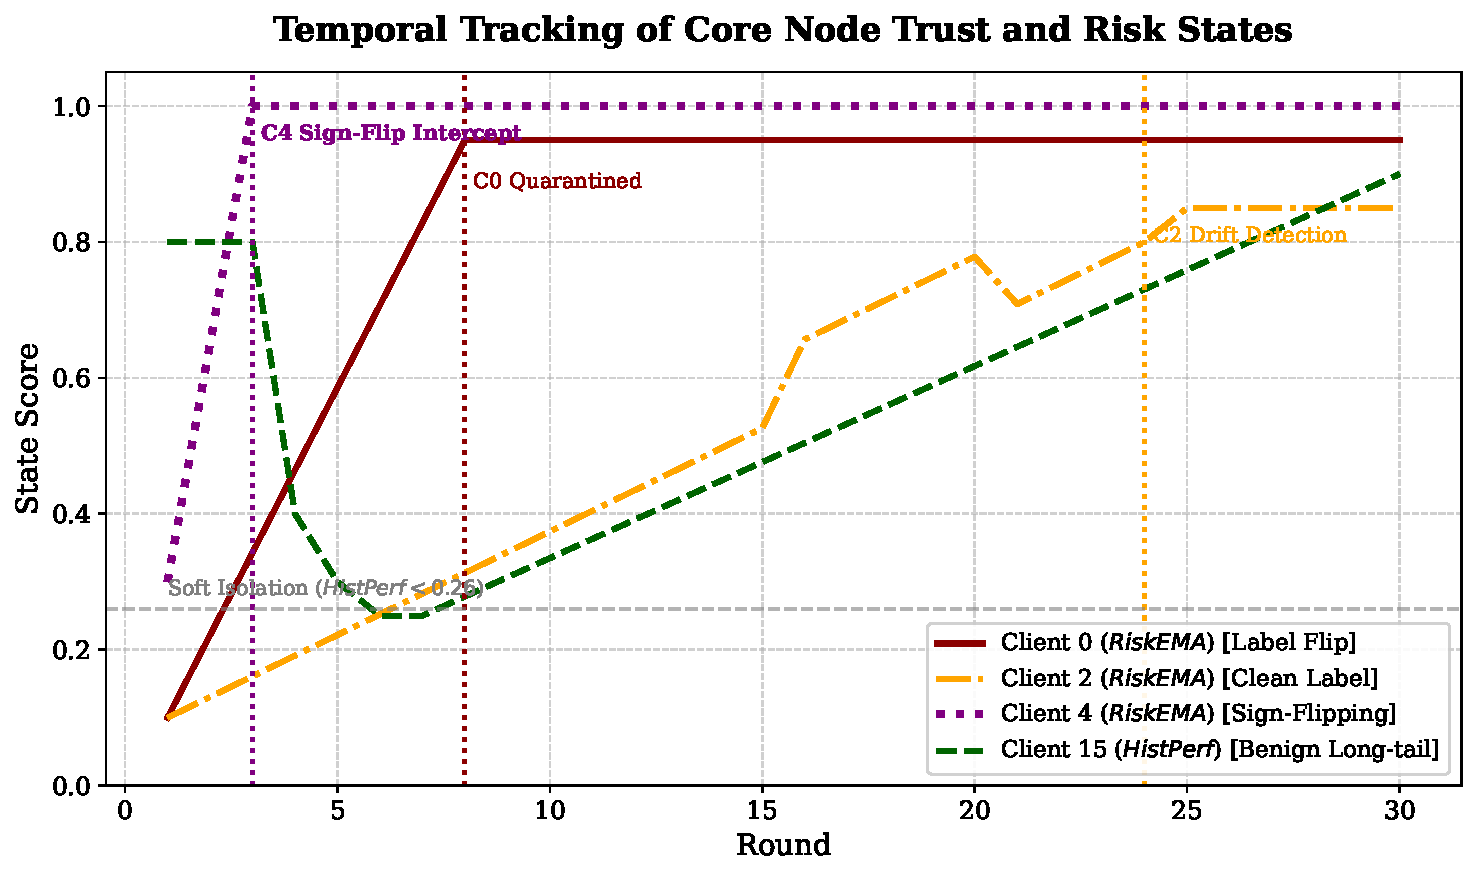
\includegraphics[width=\linewidth]{fig7_node_state_evolution.pdf}
        \vspace{-3pt}
        {\scriptsize (b) Device trust and risk trajectories.}
    \end{minipage}
    \par\vspace{6pt}
    \begin{minipage}{0.57\textwidth}
        \centering
        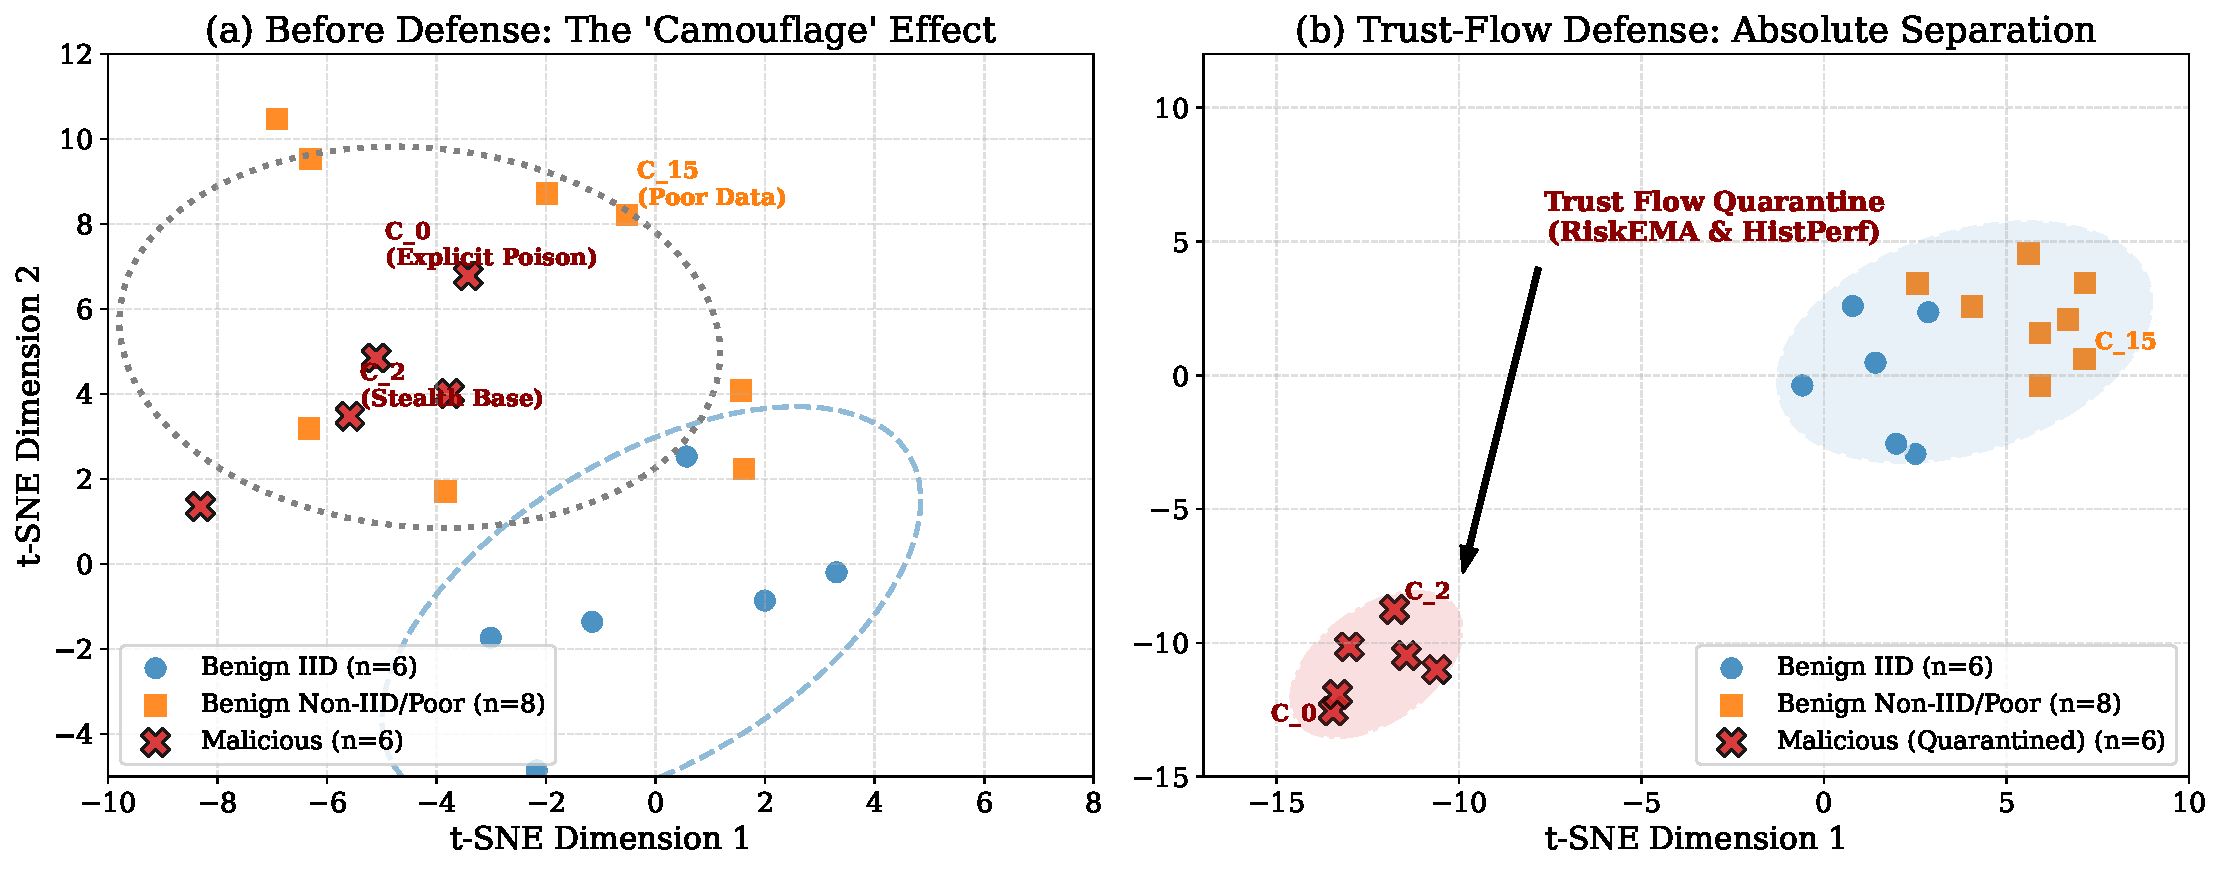
\includegraphics[width=\linewidth]{fig8_tsne_visualization.pdf}
        \vspace{-3pt}
        {\scriptsize (c) t-SNE separation before/after defense.}
    \end{minipage}
    \caption{Main defense behavior under mixed attacks.}
    \label{fig:main_results}
\end{figure}

\begin{table}[t]
    \centering
    \begin{threeparttable}
        \caption{Performance comparison under 30\% mixed attacks and boundary stress testing.}
        \label{tab:main_results}
        \scriptsize
        \setlength{\tabcolsep}{2pt}
        \begin{tabular*}{\textwidth}{@{\extracolsep{\fill}} p{2.55cm} p{2.85cm} c c c}
            \toprule
            Method/Setting & Core mechanism & Acc. & ASR & Perm. FPR \\
            \midrule
            FedAvg \cite{mcmahan2017fedavg} & no defense & $86.15\pm1.20$ & $92.34\pm5.10$ & N/A \\
            Krum \cite{blanchard2017krum} & Euclidean selection & $64.20\pm2.80$ & $12.15\pm0.90$ & $64.20$ \\
            Trimmed Mean \cite{yin2018byzantine} & coordinate trimming & $71.35\pm2.40$ & $38.60\pm4.20$ & N/A \\
            FLTrust \cite{cao2021fltrust} & clean anchor weighting & $81.25\pm1.50$ & $15.42\pm1.10$ & $21.40$ \\
            \textbf{Trust Flow} & dual stream + layered gating & $\mathbf{92.31\pm0.09}$ & $\mathbf{10.21\pm0.05}$ & $\mathbf{0.00}$ \\
            \midrule
            Boundary stress: 50\% malicious & 10/20 malicious & $91.81\pm0.10$ & $10.46\pm0.06$ & $0.00$ \\
            \bottomrule
        \end{tabular*}
        \begin{tablenotes}
            \scriptsize
            \item FPR denotes irreversible false positives for benign devices. Temporary SUSPECT/QUARANTINE states are recoverable and reported separately through trajectories.
        \end{tablenotes}
    \end{threeparttable}
\end{table}

Compared with FedAvg, robust aggregation baselines reduce ASR but either lose substantial accuracy or remove many benign long-tail devices. Krum lowers ASR to 12.15\% but its distance rule excludes many legitimate long-tail updates, leading to 64.20\% accuracy. Trimmed Mean is more stable than Krum in some rounds, yet coordinate-wise truncation cannot suppress targeted backdoor behavior sufficiently. FLTrust benefits from a clean anchor but remains vulnerable when legitimate Non-IID updates deviate from the anchor. Trust Flow preserves benign heterogeneous contributions through historical smoothing, while the short-term risk stream prevents high-reputation attackers from exploiting past behavior. In the tested 50\% stress setting, the framework retains 91.81\% accuracy and 10.46\% ASR.

\subsection{Ablation, Sensitivity, and Overhead}

Table~\ref{tab:ablation_overhead} shows that a single-stream reputation model suffers from an FPR/TPR tradeoff: aggressive thresholds increase false positives, while conservative thresholds miss sleeper attacks. HistPerf-only protects benign devices but lacks short-term attack sensitivity. The dual-stream design reaches high recall while keeping permanent false positives low in this setup. The overhead is moderate: TrustReports add about 15 KB per upload, and server aggregation time increases from 2.10 s to 4.85 s per round.

\begin{table}[t]
    \centering
    \caption{Ablation and overhead summary.}
    \label{tab:ablation_overhead}
    \scriptsize
    \setlength{\tabcolsep}{2pt}
    \begin{tabular*}{\textwidth}{@{\extracolsep{\fill}} p{2.1cm} p{4.45cm} c c}
        \toprule
        Study & Variant / architecture & FPR or overhead & TPR / time \\
        \midrule
        Reputation & Single-stream EMA, aggressive & 18.25\% FPR & 95.12\% TPR \\
        Reputation & Single-stream EMA, conservative & 2.10\% FPR & 48.33\% TPR \\
        Reputation & HistPerf-only & 0.15\% FPR & 21.05\% TPR \\
        Reputation & \textbf{Dual-stream Trust Flow} & \textbf{0.00\% FPR} & \textbf{100.00\% TPR} \\
        \midrule
        Overhead & Standard FedAvg & 0 KB extra & 2.10 s aggregation \\
        Overhead & Trust Flow & $\sim$15 KB TrustReport & 4.85 s incl. audit \\
        \bottomrule
    \end{tabular*}
\end{table}

Figures~\ref{fig:ablation_components} and \ref{fig:alpha_sensitivity} further decompose the effect of risk probes, weight re-normalization, and data heterogeneity. The FPR/TPR values in Table~\ref{tab:ablation_overhead} use the final-ban definition. Counting SUSPECT as a recoverable risk-review state gives 88.33\% per-round malicious-device coverage and a 14.79\% benign-device review trigger rate, with 0.00\% permanent false bans in the tested setting. Clean reference plus shallow probes handles sign flipping and gradient scaling, but Clean-Label Backdoor attacks remain difficult when gradient directions are collinear with benign updates. Adding cross-entropy and high-level activation probes reduces clean-label ASR below 9.2\%. Re-normalization also matters: layer-wise gating without survivor weight correction creates an implicit learning-rate decay, while full Trust Flow converges within the 30-round budget. Under Dirichlet $\alpha=0.1$, Krum and FLTrust degrade sharply, whereas Trust Flow remains near 92\% accuracy.

The sensitivity curve confirms that traditional robust aggregation behaves well when data are close to IID, but deteriorates as $\alpha$ decreases. With $\alpha=100$ or $\alpha=1.0$, Krum and FLTrust remain close to the proposed method. In the long-tail setting $\alpha=0.1$, however, their filtering rules increasingly treat legitimate drift as malicious deviation. Trust Flow is less sensitive to this shift because content evidence is not used alone; it is integrated with historical utility and short-term risk. The fusion parameter $\beta_{fusion}$ controls how strongly the clean reference dominates peer consistency. A smaller value retains more long-tail devices but raises ASR, while a larger value improves attack suppression but can over-penalize heterogeneous updates. The default $\beta_{fusion}=2.0$ provides the best observed Acc/ASR balance.

The overhead analysis indicates that Trust Flow mainly shifts cost to the server. The embodied device side appends a TrustReport of roughly 15 KB and performs lightweight runtime monitoring. The server performs reference construction, pairwise consistency auditing, dual-stream updates, and layer-wise clipping, increasing aggregation time from 2.10 s to 4.85 s in the tested setup. Because wide-area embodied FL rounds usually spend far more time on communication and synchronization than on aggregation arithmetic, this increase remains acceptable for the target scenario.

\begin{figure}[t]
    \centering
    \begin{minipage}{0.49\textwidth}
        \centering
        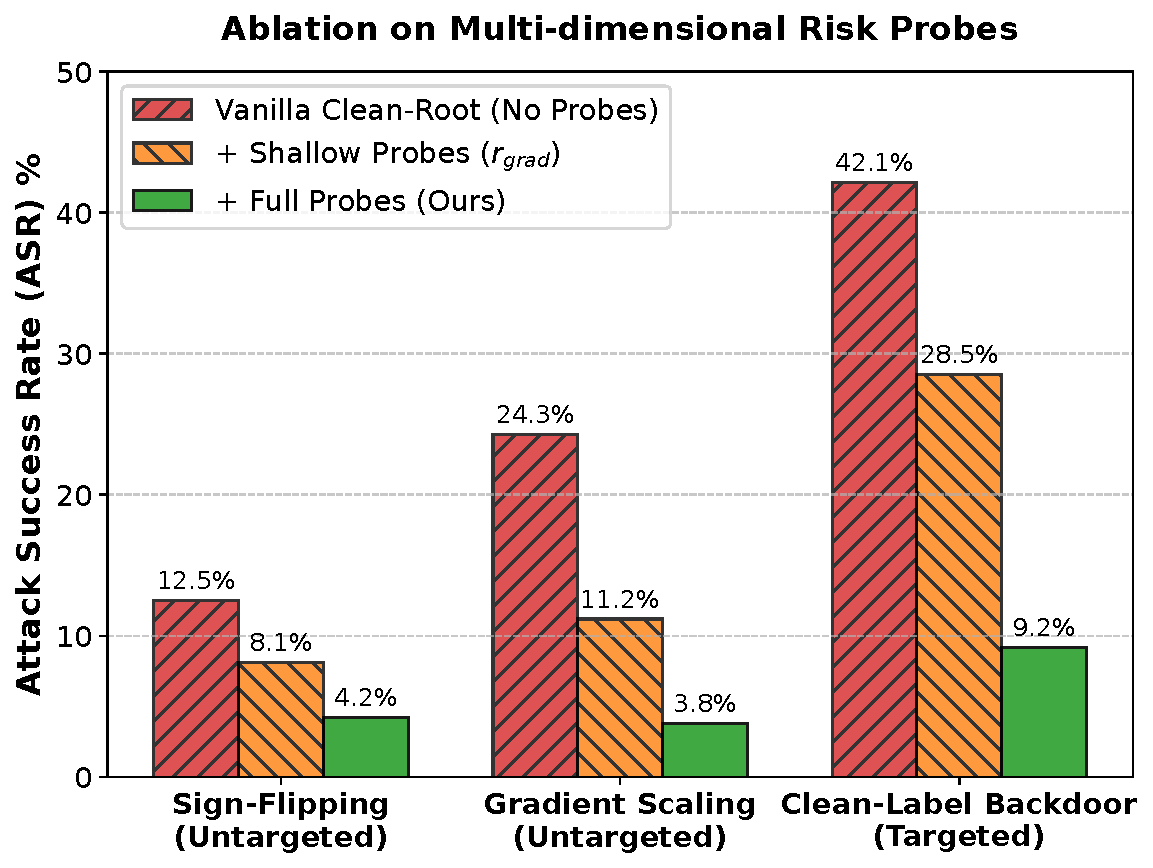
\includegraphics[width=\linewidth]{fig9_ablation_probes.pdf}
        \vspace{-3pt}
        {\scriptsize (a) Multi-dimensional risk-probe ablation.}
    \end{minipage}\hfill
    \begin{minipage}{0.49\textwidth}
        \centering
        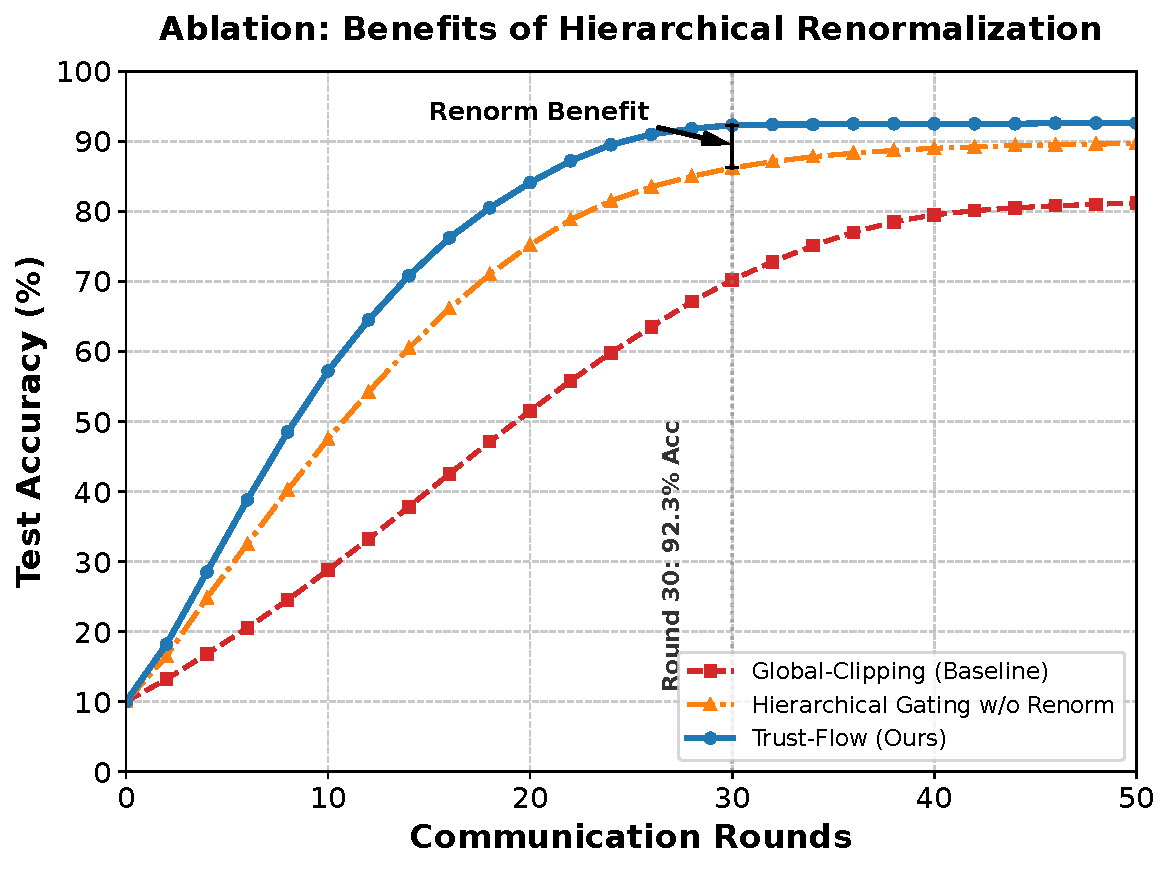
\includegraphics[width=\linewidth]{fig10_ablation_renorm.pdf}
        \vspace{-3pt}
        {\scriptsize (b) Weight re-normalization effect.}
    \end{minipage}
    \caption{Component-level ablation of risk probes and re-normalization.}
    \label{fig:ablation_components}
\end{figure}

\begin{figure}[t]
    \centering
    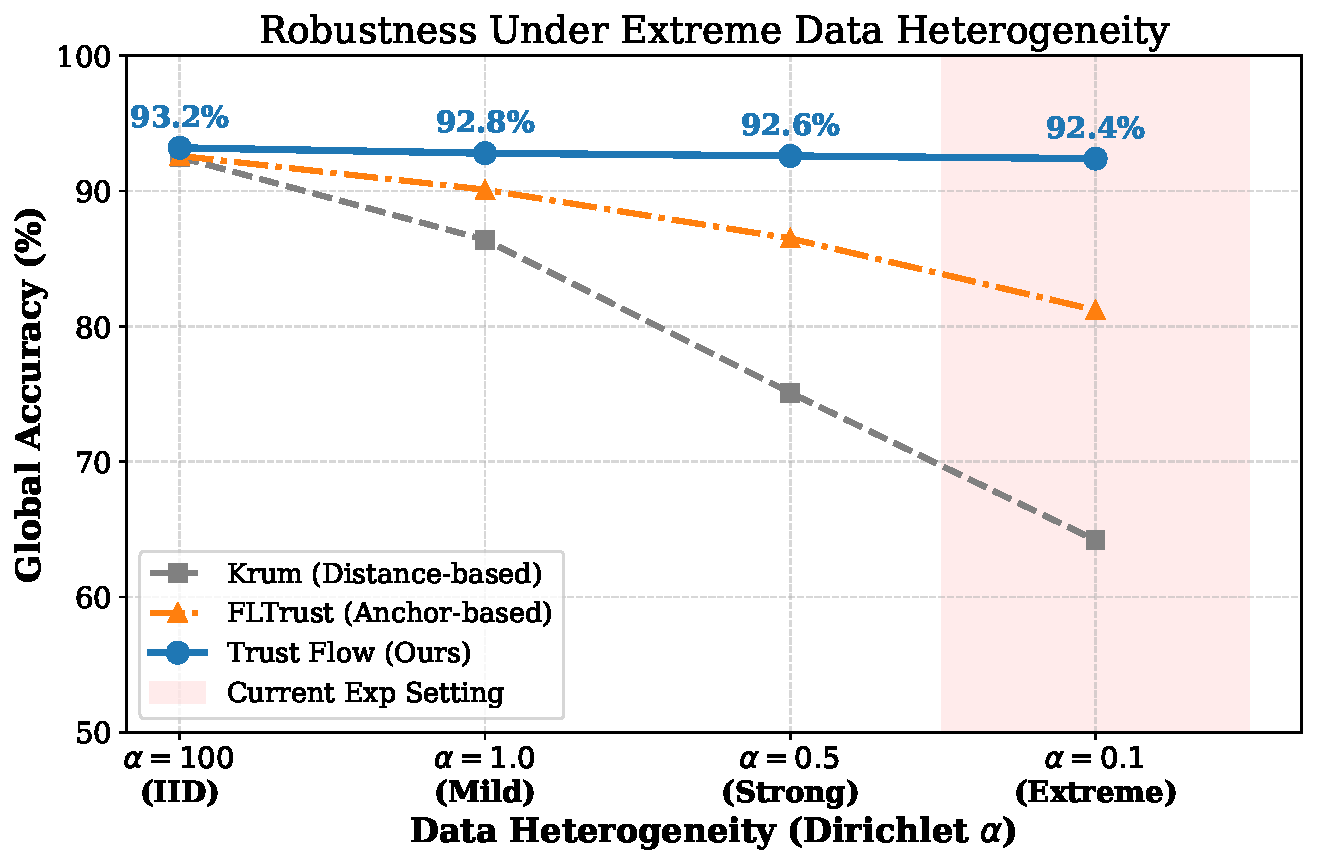
\includegraphics[width=0.76\textwidth]{fig11_alpha_sensitivity.pdf}
    \caption{Robustness stress test under varying data heterogeneity.}
    \label{fig:alpha_sensitivity}
\end{figure}

\section{Discussion and Conclusion}

Trust Flow integrates admission evidence, content auditing, temporal reputation, and layer-wise aggregation into a single trust-state pipeline for embodied AI edge collaboration. Its main benefit is a cleaner separation between benign long-tail drift and malicious manipulation, which keeps permanent-ban FPR low in the reported experiments while maintaining high recall against mixed attacks.

Several limitations remain. Some emerging TEE-FL methods lack publicly verifiable implementations, so this study does not include them as direct baselines. The current probe design is also tailored to vision classification. Future work will release source code and scripts, evaluate larger embodied edge deployments, and extend the multidimensional risk probes to multimodal embodied models, NLP, and federated fine-tuning.

\begingroup
\small
\begin{thebibliography}{99}
    \setlength{\itemsep}{0pt}
    \bibitem{kairouz2021flsurvey} Kairouz, P., McMahan, H.B., Avent, B., et al.: Advances and open problems in federated learning. Foundations and Trends in Machine Learning 14(1--2), 1--210 (2021). \url{https://doi.org/10.1561/2200000083}
    \bibitem{mcmahan2017fedavg} McMahan, B., Moore, E., Ramage, D., Hampson, S., Aguera y Arcas, B.: Communication-efficient learning of deep networks from decentralized data. In: Proceedings of the 20th International Conference on Artificial Intelligence and Statistics, PMLR 54, pp. 1273--1282 (2017). \url{https://proceedings.mlr.press/v54/mcmahan17a.html}
    \bibitem{blanchard2017krum} Blanchard, P., El Mhamdi, E.M., Guerraoui, R., Stainer, J.: Machine learning with adversaries: Byzantine tolerant gradient descent. In: Advances in Neural Information Processing Systems 30 (2017). \href{https://papers.nips.cc/paper/6617-machine-learning-with-adversaries-byzantine-tolerant-gradient-descent}{NeurIPS paper page}
    \bibitem{yin2018byzantine} Yin, D., Chen, Y., Ramchandran, K., Bartlett, P.: Byzantine-robust distributed learning: Towards optimal statistical rates. In: Proceedings of the 35th International Conference on Machine Learning, PMLR 80, pp. 5650--5659 (2018). \url{https://proceedings.mlr.press/v80/yin18a.html}
    \bibitem{cao2021fltrust} Cao, X., Fang, M., Liu, J., Gong, N.Z.: FLTrust: Byzantine-robust federated learning via trust bootstrapping. In: Proceedings 2021 Network and Distributed System Security Symposium (NDSS) (2021). \url{https://doi.org/10.14722/ndss.2021.24434}
    \bibitem{fung2020foolsgold} Fung, C., Yoon, C.J.M., Beschastnikh, I.: The limitations of federated learning in Sybil settings. In: 23rd International Symposium on Research in Attacks, Intrusions and Defenses (RAID 2020), pp. 301--316. USENIX Association (2020). \url{https://www.usenix.org/conference/raid2020/presentation/fung}
    \bibitem{wang2025rasa} Wang, L., Huang, M., Zhang, Z., Li, M., Wang, J., Gai, K.: RaSA: Robust and adaptive secure aggregation for edge-assisted hierarchical federated learning. IEEE Transactions on Information Forensics and Security 20, 4280--4295 (2025). \url{https://doi.org/10.1109/TIFS.2025.3559411}
    \bibitem{fldetector2022} Zhang, Z., Cao, X., Jia, J., Gong, N.Z.: FLDetector: Defending federated learning against model poisoning attacks via detecting malicious clients. In: Proceedings of the 28th ACM SIGKDD Conference on Knowledge Discovery and Data Mining, pp. 2545--2555 (2022). \url{https://doi.org/10.1145/3534678.3539231}
    \bibitem{deepsight2022} Rieger, P., Nguyen, T.D., Miettinen, M., Sadeghi, A.R.: DeepSight: Mitigating backdoor attacks in federated learning through deep model inspection. In: Network and Distributed System Security Symposium (NDSS) (2022). \url{https://doi.org/10.14722/ndss.2022.23156}
    \bibitem{flame2022} Nguyen, T.D., Rieger, P., Chen, H., et al.: FLAME: Taming backdoors in federated learning. In: 31st USENIX Security Symposium, pp. 1415--1432 (2022). \url{https://www.usenix.org/conference/usenixsecurity22/presentation/nguyen}
    \bibitem{flpurifier} Zhang, J., Zhu, C., Sun, X., Ge, C., Chen, B., Susilo, W., Yu, S.: FLPurifier: Backdoor defense in federated learning via decoupled contrastive training. IEEE Transactions on Information Forensics and Security 19, 4752--4766 (2024). \url{https://doi.org/10.1109/TIFS.2024.3384846}
    \bibitem{crowdguard2024} Rieger, P., Krau{\ss}, T., Miettinen, M., Dmitrienko, A., Sadeghi, A.R.: CrowdGuard: Federated backdoor detection in federated learning. In: Network and Distributed System Security Symposium (NDSS) (2024). \url{https://doi.org/10.14722/ndss.2024.23233}
    \bibitem{roseagg} Yang, H., Xi, W., Shen, Y., Wu, C., Zhao, J.: RoseAgg: Robust defense against targeted collusion attacks in federated learning. IEEE Transactions on Information Forensics and Security 19, 2951--2966 (2024). \url{https://doi.org/10.1109/TIFS.2024.3352415}
    \bibitem{shieldfl} Ma, Z., Ma, J., Miao, Y., Li, Y., Deng, R.H.: ShieldFL: Mitigating model poisoning attacks in privacy-preserving federated learning. IEEE Transactions on Information Forensics and Security 17, 1639--1654 (2022). \url{https://doi.org/10.1109/TIFS.2022.3169918}
    \bibitem{r1_tee_integrity} Chen, Y., Luo, F., Li, T., Xiang, T., Liu, Z., Li, J.: A training-integrity privacy-preserving federated learning scheme with trusted execution environment. Information Sciences 522, 69--79 (2020). \url{https://doi.org/10.1016/j.ins.2020.02.037}
    \bibitem{xu2021distributed} Xu, T., Zhu, K., Andrzejak, A., Zhang, L.: Distributed learning in trusted execution environment: A case study of federated learning in SGX. In: 2021 7th IEEE International Conference on Network Intelligence and Digital Content (IC-NIDC), pp. 450--454 (2021). \url{https://doi.org/10.1109/IC-NIDC54101.2021.9660433}
    \bibitem{zhang2025rppfl} Zhang, X., Chen, Z., Chen, G., Feng, X., Shen, Q., Wu, Z.: RPPFL: Robust and privacy-preserving federated learning via trusted execution environments. In: ICASSP 2025 - 2025 IEEE International Conference on Acoustics, Speech and Signal Processing, pp. 1--5 (2025). \url{https://doi.org/10.1109/ICASSP49660.2025.10889398}
    \bibitem{r5_tee_mitigating} Queyrut, S., Schiavoni, V., Felber, P.: Mitigating adversarial attacks in federated learning with trusted execution environments. In: 2023 IEEE 43rd International Conference on Distributed Computing Systems (ICDCS), pp. 626--637 (2023). \url{https://doi.org/10.1109/ICDCS57875.2023.00069}
    \bibitem{lu2025tmt} Lu, Z., Wang, L., Zhang, Z., Huang, M., Wang, J., Li, M.: TMT-FL: Enabling trustworthy model training of federated learning with malicious participants. IEEE Transactions on Dependable and Secure Computing 22(3), 2723--2740 (2025). \url{https://doi.org/10.1109/TDSC.2024.3521377}

    \bibitem{bagdasaryan2020backdoor} Bagdasaryan, E., Veit, A., Hua, Y., Estrin, D., Shmatikov, V.: How To Backdoor Federated Learning. In: Proceedings of the Twenty Third International Conference on Artificial Intelligence and Statistics, PMLR 108, pp. 2938--2948 (2020). \url{https://proceedings.mlr.press/v108/bagdasaryan20a.html}
    \bibitem{wang2019neuralcleanse} Wang, B., Yao, Y., Shan, S., Li, H., Viswanath, B., Zheng, H., Zhao, B.Y.: Neural Cleanse: Identifying and mitigating backdoor attacks in neural networks. In: 2019 IEEE Symposium on Security and Privacy (SP), pp. 707--723 (2019). \url{https://doi.org/10.1109/SP.2019.00031}

\end{thebibliography}
\endgroup

\end{document}
